% !TEX root = ../main.tex

\section{Experimental Setup}
\label{sec:orgb44ba25}

We test the effect of optimizing using our proposed sigmoidF1 loss function on four datasets across different modalities, namely image and text. %with a focus on text: the most comparable research was on text data. 
The datasets share that the full instance (the entire image or the full text) is predictive of its labels. The next section and Table~\ref{table:datasets} describe our four datasets in detail.

% \doubt{optional paragraph}
% In light of the problem definition leading to the sigmoidF1 framework in the introduction and in order to clearly delimit the proposed method, following are a few datasets that are not suitable for the task.

\subsection{Datasets}

\todo{see if related work section comes before this and introduces ML-NET}\daan{I think we are not moving related work to the front again.}

Our first dataset comes from the vision domain and consists of a dataset of movie posters and their genre (e.g. \emph{action}, \emph{comedy})\footnote{Labels available at https://tinyurl.com/y7ydyedu and prescraped images from IMDB at https://tinyurl.com/y7lfpvlx}. The posters and labels have been extracted from IMDB and the dataset was previously used for \todo{XXX and cite}. The genre labels in this dataset are not mutually exclusive and of varying counts per movie. 

For a broad scope in learning for text, we use the newly created \emph{arXiv dataset}\footnote{Available at \url{https://www.kaggle.com/Cornell-University/arxiv}} with over 1.7 million open source articles and their metadata. Our experiments use the abstracts and categories, that are suitably mutually inclusive and have a varying count per example. There is a longer history of using arXiv to create research datasets. The dataset we use is not to be confused with an earlier long document dataset that that only features 11 classes \cite{oldarXiv}, but was used in a recent long transformer publication~\cite{bigBird}. The limited number of labeled classes render this dataset not suited for our experiments.  We denote \textit{arXiv2020} as the subset of the \emph{arXiv dataset} with only documents published in 2020, given limited computing power. This results in around 26k documents.

ML-NET~\cite{multitaskLabel} is the state-of-the-art in \emph{fit-algorithm-to-data} for text to the best of our knowledge. Among the three datasets used for benchmarking ML-NET, the cancerHallmark~\cite{cancerHallmarks}\footnote{Available at \url{https://github.com/sb895/Hallmarks-of-Cancer}} and chemicalExposure~\cite{chemExposure}\footnote{Available at \url{https://github.com/sb895/chemical-exposure-information-corpus}} datasets are of multi-instance multilabel nature: several expressions are annotated within each paper abstracts. The third dataset diagnosisCodes could not be recovered, upon contacting the authors of both ML-NET and the original paper~\cite{diagnosisCode}. 

\begin{table}
\caption{Descriptive statistics of our experimental datasets.}
\label{table:datasets}
\centering
% \begin{adjustbox}{max width=\textwidth}
\begin{tabular}{l ccccc}
\toprule
& & & Average & Number of \\
& Type & Classes & label count & examples \\
\midrule
moviePosters & image & 28 & 2.165 & 37632\\
arXiv2020 & text & 155 & 1.888 & 26558\\ 
chemExposure & text & 38 & 6.116 & 3661\\
cancerHallmarks\hspace{-.7em}  & text & 33 & 3.501 & 1582\\
\bottomrule
\end{tabular}
% \end{adjustbox}
\end{table}

\subsection{Learning Framework}

The learning framework consists of two parts: a pretrained deep neural network and a classification head (see Figure \ref{fig:architecture}). We performed our experiments on Amazon Web Services cloud machines with parallelization on up to 16 GPUs \textit{p2.16xlarge}, with TensorFlow 2 as a gradient-descent backend.

\begin{figure*}[htbp]
\centering
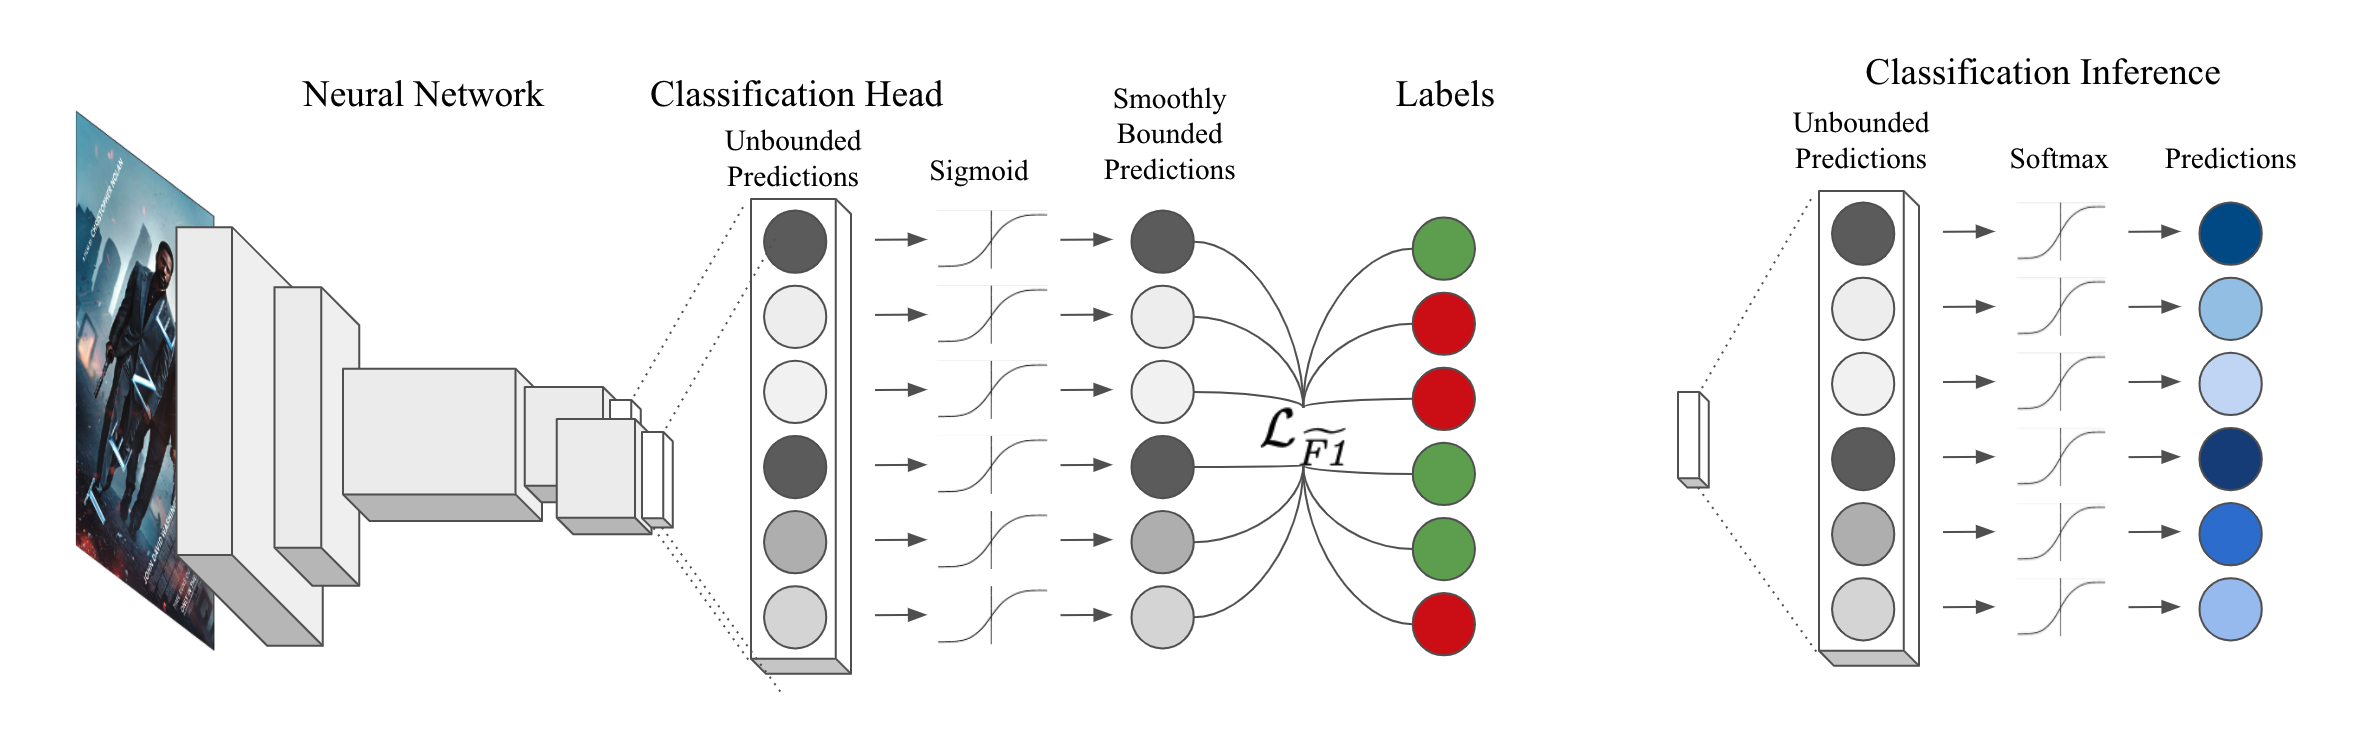
\includegraphics[width=.9\linewidth]{./images/architecture.png}
\caption{\label{fig:architecture}
Pretrained Network and Classification Head for sigmoidF1 \todo{some tweaks}}
\end{figure*}

Since the focus of this paper is in comparing loss functions and not neural network architectures, we chose efficient network architectures in terms of accuracy and computation.
For the moviePoster image dataset, we use a MobileNetV2~\cite{mobileNet} architecture that was pretrained on ImageNet~\cite{imagenet}. This network architecture is typically used for inference on small computing devices (e.g. smartphones). We use a version of MobileNetV2 already stripped off of its original classification head.\footnote{The pretrained network can be loaded here \url{https://tfhub.dev/google/imagenet/mobilenet_v2_100_224/feature_vector/4}}
For the three text datasets, we use DistilBert~\cite{distilBert} as implemented in Hugging Face. This is a particularly efficient instance of the BERT model\footnote{The pretrained network can be loaded here \url{https://huggingface.co/transformers/model_doc/distilbert.html}}. 
In both cases, we use the final pretrained layer as an embedding of the input. In order to make sure that the results of different loss functions are comparable, we fix the model weights of the pretrained CNN and DistilBert and keep the hyperparameter values that were used to train them from scratch. We also use the same TensorFlow internal random seeds.

A similar classification head is used for both models. It consists of a latent representation layer (the final pretrained layer mentioned above) connected with a RELU activation. This layer is linked to a final classification layer with a linear activation. The dimension of the final layer is equal to the number of classes in the dataset. When computing focalLoss and crossEntropy, a softmax transformation transforms the unbounded last layer to a $[0,1]$ bounded vector. When computing sigmoidF1 loss, a sigmoid transformation is operated instead, which results in a sparser $[0,1]$ vector. At inference time, the last layer is used for prediction and is bounded with a softmax function. A threshold must then be chosen at evaluation time to compute different metrics. Figure \ref{fig:architecture} depicts this learning framework.

% \footnote{Original tencentLoss is available at \url{https://github.com/Tencent/tencent-ml-images/blob/master/train.py}. We ported this to TensorFlow 2 and share this at ANONYMIZED.},

\subsection{Hyperparameters and Reproducibility}

We choose to ignore classes that are underrepresented, in order to give the model a fair chance at learning from at least a few examples. We define underrepresentation as a global irrelevance threshold $b$ for classes: any class $c$ that is represented less than $b$ times is considered irrelevant. We decided to set an irrelevance threshold $b$ on all datasets prior to conducting experiments, so as to not finetune for that feature. It was set to 1000 for both \emph{arXiv2020} (145 of the \todo{XXX} classes remaining) and \emph{moviePosters} (14 of the \todo{XXX} classes remaining) and at 10 for \emph{chemicalExposure} and \emph{cancerHallmarks}, in proportion to the number of classes and labels in each dataset. The sensitivity study below illustrates what happens when we let $t$ vary over the arXiv2020 dataset.
\todo{fill in in remaining classes for medical datasets}

Batch size is set at a high value of 256. We thus increase accuracy over traditional losses~\cite{bigBS}, but also allow heterogeneity in the examples within the batch, thus collecting enough values in each quadrant of the confusion matrix. In a future research, it would be interesting to establish the minimum required batch size for sigmoidF1. \daan{I think we should discuss this need for a large batch size in a bit more detail in 3 and then we can reference that here and say we set it sufficiently high. We really should have an experiment with this parameter, but there is no time to still run that.}

Regarding the sigmoidF1 hyperparameters $\beta$ and $\eta$, we performed a grid search with the values in the \todo{regions $[1;30]$ and $[0;2]$}\daan{exact values here} respectively. In our experiments, we evaluate the sensitivity of our method to these hyperparameters (see Figure \ref{fig:sigmoid}). Note that negative values of $\beta$ geometrically reflect the sigmoid function across the horizontal line at $0.5$ and thus invert predictions. \daan{Should this last sentence not be in 3?}

We made sure to split the data in the same train, validation and test sets for each different loss function. You can download our code to retrieve the exact train, valid and test sets. The next section details the result of the experiments on the test set.
\gab{are the terms train, valid and test, used in IR? I see a lot of papers use the term dev set as well instead of test set} \daan{this is clear, do not worry.}

% \subsection{Inference Time}

% As illustrated in the previous section, there are different ways of compounding metrics over each class for multilabel classification (mainly, micro, macro and weighted metrics). Certain loss functions such as focal loss and  For the sake of Macro compounding was used on all loss functions, since certain 

% Cancer can be described according to its complexity with different principles, named hallmarks cite:cancerHallmarks. A corpus of 1580 PubMed abstracts are manually annotated for 10 hallmarks. This is a multi-instance labelling task and will therefore not be used here.

% [[./images/cancerHallmarksAnnotation.jpg]]

% - Multilabel classification for text cite:toxicComments

% - Scenery dataset for images cite:dataScenery.

% \todo{this is an ambitious number of datasets. Add longer description of each dataset, depending on which ones I keep: sample size, number of classes etc. see utils here: https://github.com/ashrefm/multi-label-soft-f1}

\subsection{Evaluation Metrics}
\label{sec:org23c8447}

In our experimental evaluation, we consider a suite of metrics that are commonly used in the evaluation of multilabel classification to measure the effectiveness of multilabel prediction. Such metrics are based on the confusion matrix, which we detailed in Section~\ref{section:method} and for which we provided smoothed surrogates to optimize directly.

When true positives and false positives are used, recall that \(t p=\sum_{i \in Y^{+}} \mathds{1}_{\mathbf{p_i} \geq t}\) and \(f p=\sum_{i \in Y^{-}} \mathds{1}_{\mathbf{p_i} \geq t}\), and thus a threshold \(t\) must be set. When \(t = 0.5\), as is commonly done \todo{add source}, a risk remains that a lot of examples remain without predictions. \daan{Sharpen this end defend our choices.}
Note that for the two medical datasets cancerHallmarks and chemicalExposure, information is a lot more sparse, we thus set the evaluation metrics threshold at 0.05 and train for 500 epochs until reaching convergence. 

Extending \(F_1\) to multi-class binary classification amounts to deciding wether or not to pool classes.
In a first pooled iteration, micro \(F_1\)~\cite{multilabelMetrics} equates to creating a single 2x2 confusion matrix for all classes:
$$F_1^{micro} = \frac{\sum tp_c}{2 \sum tp_c + \sum fn_c + \sum fp_c} \quad for \quad c \in C$$

Macro \(F_1\) \cite{threshForF1, multilabelMetrics} amounts to creating one confusion matrix per class or unpooling:

$$F_1^{macro} = \frac{1}{c} \sum_{j=1}^c F_1$$

% $$F_1^{macro} = \frac{\sum tp_c}{2 \sum tp_c + \sum fn_c + \sum fp_c} \quad for \quad c \in C$$

Weighted macro \(F_1\)~\cite{weightedMetrics} is similar but includes weighing to account for class imbalance, i.e. weighing each class by the number of groundtruth positives.
\begin{equation}
F_1^{weighted} = \frac{1}{c} \sum_{j=1}^c n_j F_1 \text{ where } n_j = \sum_i \mathds{1}_{\mathbf{y_i^j} = 1}.
\end{equation}

% $$F_1^{weighted} = \frac{\sum tp_c}{2 \sum tp_c + \sum fn_c + \sum fp_c} \quad for \quad c \in C$$

We also define precision and recall

\begin{equation}
\begin{aligned} P &=\frac{t p}{t p+f p} \\ R &=\frac{t p}{t p+f n}=\frac{t p}{\left|Y^{+}\right|} \end{aligned}
\end{equation}

More variations scores exist in the literature, such as hamming loss~\cite{hammingLoss} (the fraction of incorrectly predicted labels), \todo{hamming score}.\daan{As this is a loss, should it not go to related?}

In our experiments, we report on macroF1, microF1, weightedF1, Precision and Recall. We focus our discussion of experimental result around weightedF1 as we consider this the most representative for success on FIMPUL problems. 
\daan{I want so say something like below. Please see if you agree.}
We point out that there is an interaction between our optimization on sigmoidF1 and our evaluation using F1 metrics. If our approach of optimizing for an F1 surrogate succeed, we expect higher values on F1-related metrics during evaluation. For this reason, we consider and discuss not a single, but multiple metrics.

% - 'samples':
% Calculate metrics for each instance, and find their average (only meaningful for multilabel classification where this differs from accuracy_score).

% $$F_1^{micro} = \frac{\sum tp_c}{2 \sum tp_c + \sum fn_c + \sum fp_c} \quad for \quad c \in C$$



%%% Local Variables:
%%% mode: plain-tex
%%% TeX-master: "../meta"
%%% End:
